%%%%%%%%%%%%%%%%%%%%%%%%%%%%%%%%%%%%%%%%%%%%%%%%%%%%
\section{Preliminaries}\label{sec:preliminaries}
%%%%%%%%%%%%%%%%%%%%%%%%%%%%%%%%%%%%%%%%%%%%%%%%%%%%

\subsection{BDI Agent-Oriented Programming}\label{sec:bdi_programming}

\notems{new para}
BDI agent-oriented programming is a popular, well-studied, and practical paradigm
for building intelligent agents situated in complex and dynamic environments with
(soft) real-time reasoning and control requirements
\cite{Georgeff89-PRS,Benfield:AAMAS06}.
% %
Generally speaking, BDI agent-oriented programming languages are built around an
explicit representation of propositional attitudes (e.g., beliefs, desires,
intentions, etc.). A BDI architecture addresses how these components are
represented, updated, and processed to determine the agent's actions.
% .
There are a number of agent programming languages and development platforms in
the BDI tradition, such as \PRS~\cite{IngrandGR:IEEE92-PRS} and
\dMARS~\cite{Inverno:JAAMAS04-dMARS}, \AgentSpeak\ and
\JASON~\cite{Rao:LNCS96-AgentSpeak,Bordini:07-JASONBOOK},
\JADEX~\cite{PokahrBL:EXP03-JADEX},
\TAPL~\cite{Hindriks:JAAMAS99-3APL,DastaniRM:05} and
\DAPL~\cite{Dastani:JAAMAS08-2APL}, \GOAL~\cite{BoerHHM:JAPL07-GOAL},
\JACK~\cite{BusettaRHL:AL99-JACK}, SRI's \SPARK~\cite{MorelyM:AAMAS04-SPARK}, and
\JAM~\cite{Huber:AGENTS99-JAM}.


\begin{figure}[t]
\begin{center}
\resizebox{\textwidth}{!}{\begin{tikzpicture}

\tikzstyle{centityd}=[draw=black]
\tikzstyle{centityf}=[fill=black!20]
\tikzstyle{centity}=[centityd,centityf]
\tikzstyle{entity}=[centity,thick,text centered,anchor=center]


\node[anchor=east] at (6,4.5)  {dynamic};
\node[anchor=west] at (7,4.5) {static};


\node (database) at (1,8.8)  (B)
	[cylinder,entity,shape border rotate=90,minimum width=1.6cm,shape aspect=.3]
	{\textbf{Beliefs}};


\node  (environment)  
       [below left of=B, rounded corners, minimum height=3cm,
       starburst,fill=black!10,rotate=90,shift={(-1cm,4cm)}] 
       {\textbf{\large Environment}};



\node at (4,10) (eventQueue) {{\bf Pending Events}};
\begin{pgfonlayer}{foreground}
\foreach \x in {3.5,3.7,...,4.5}
\draw [fill=black!50](\x,9.2) circle (0.2);
\end{pgfonlayer}
%\path (4,9.1) node (Q) {}; 
\draw (4,9.2) node (Q) 
	[entity, text width=1.4cm, minimum height=0.8cm] {};




\foreach \x in {4,3,2,1}
\draw (-.6,5) node (I) [anchor=south,draw, centity, text width=.5em,
	minimum height=\x em]{};
\foreach \x in {3,2,1}
\draw (0.2,5) node (I) [anchor=south,draw,centity, text width=.5em,
	minimum height=\x em]{};
\foreach \x in {5,4,3,2,1}
\draw (1,5) node (I) [anchor=south,draw, centity, text width=0.5em,
	minimum height=\x em]{};
\node[below left of=I] (Intentions) {{\bf  Intention Stacks}};


% { [start chain=1]
% % \node [on chain,draw] at (0,6) {};
%     \foreach \x in {1,2,...,11} {
%        \x, \node [draw,on chain=1] {};
%     }
% }

\begin{pgfonlayer}{foreground}
\node[anchor=center] at (4,6)  (deli) 
	{\begin{tabular}{c}
     	\textbf{BDI engine} 
     \end{tabular}};
\node at (4,3.4) (actions) {{\bf actions}};
\node at (2.5,11.4) [starburst,centityd] (in) {{\bf events}};


\draw node (P) 
	[right of=deli,xshift=3cm,rounded corners, double copy
	shadow={opacity=0.8},text centered, entity, minimum height=5em] 
	{	\begin{tabular}{c} 
          \textbf{Plan} \\[1ex]
          \textbf{library}
         \end{tabular}	};



\draw[thick,->] (in) -- (B) ; 
\draw[thick,->] (in) -- (eventQueue) ; 
\draw[thick,->] (deli) -- (actions) ; 
\draw[thick,<->] (deli) -- (I) ; 
\draw[thick,<->] (deli) -- (B) ; 
\draw[thick,<-] (deli) -- (P) ;
\draw[thick,<->] (deli) -- (Q) ; 
\end{pgfonlayer}








\begin{pgfonlayer}{background}

%% Dotted box encapuslating the agent
\path (-1.5,10.5) node (c) {};
\path (9.5,4) node (d) {};
\path[fill=none,rounded corners, draw=black!50, dashed] (c) rectangle (d);




\draw[->,very thick,dashed] (environment) 
		|- node[above,xshift=1cm] {SENSORS}
	 	(in);
\draw[->,very thick,dashed] (actions.west) 
		-| node[below,xshift=1cm] {ACTUATORS}
		(environment.west);
\end{pgfonlayer}


\foreach \x in {-9,9,...,360}
\fill [rotate around={\x:(3.2,5.6)},centityf] 
	(4.0,5.4743) -- (4.2 ,5.6) -- (4.0,5.7257) -- (4.0,5.3487);
\fill [centityf] (3.2,5.6) circle (0.8);

\foreach \x in {0,18,...,360}
\fill [rotate around={\x:(4.8,6.4)},centityf] 
	(5.6,6.2743)-- (5.8,6.4) -- (5.6,6.5257) -- (5.6,6.2743);
\fill [centityf] (4.8,6.4) circle (0.8);


\end{tikzpicture}}
\end{center}
\caption{A typical BDI-style architecture}
\label{fig:bdiarch}
\end{figure}

In a BDI-style system, an agent consists, basically, of a belief base (akin to a
database), a set of recorded pending goal events, a plan library, and an
intention base. 
%%
Figure~\ref{fig:bdiarch} depicts a typical BDI architecture.
%%
While the belief base encodes the agent's knowledge about the
world, the pending events stand for the \emph{goals} the agent wants to
achieve/resolve.
% %
The \textit{plan library}, in turn, contains \emph{plan rules}, or simply
\emph{plans}, of the general form $e: \psi \leftarrow \delta$ encoding the
standard domain operational procedure $\delta$ (that is, a program) for achieving
the event-goal $e$ when the so-called \textit{context condition} $\psi$ is
believed true---program $\delta$ is a reasonable strategy to resolve event $e$
whenever $\psi$ holds. Among other operations, the plan-body program $\delta$
will typically include the execution of actions ($act$) in the environment and
subgoal events ($!e$) that ought to be in turn resolved by selecting suitable
plans for that subgoal event. Lastly, the intention base accounts for the
current, partially instantiated, plans that the agent has already committed to in
order to handle or achieve some event-goal.


The basic reactive goal-oriented behavior of BDI systems involves the system
responding to events, the inputs to the system, by committing to handle one
pending event-goal, \textit{selecting a plan} from the library, and placing its
program body  into the intention base.
% %%
A plan may be selected if it is \textit{relevant} and \textit{applicable}, that is, if it
is a plan designed for the event in question and its context condition is
believed true, respectively.
% %
In contrast with traditional planning, execution happens at each step. The
assumption is that the use of plans' context-preconditions to make choices as
late as possible, together with the built-in goal-failure mechanisms, ensures
that a successful execution will eventually be obtained while the system is
sufficiently responsive to changes in the environment.


For the purposes of this paper, we shall mostly focus on the plan library, as we
investigate ways of learning how agents can make a better use of it over time.
% %
It is not hard to see that, by grouping together plans responding to the same
event type, the plan library can be seen as a set of \emph{goal-plan tree}
templates: a goal (or event) node has children representing the alternative
relevant plans for achieving it; and a plan node, in turn, has children nodes
representing the subgoals (including primitive actions) of the plan.
% %%
These structures, can be seen as AND/OR trees: for a plan to succeed all the
subgoals and actions of the plan must be successful (AND); for a subgoal to
succeed one of the plans to achieve it must succeed (OR).

Consider, for instance, the structure depicted in
Figure~\ref{fig:T3}.
% %%
A link from a goal to a plan means that this plan is relevant (i.e., potentially
suitable) for achieving the goal (e.g., $P_1 \ldots P4$ are the relevant
plans for event goal $G$); whereas a link from a plan to a goal means that the
plan needs to achieve that goal as part of its (sequential) execution (e.g., plan
$P_A$ needs to achieve goal $G_{A1}$ first and then $G_{A2}$).
% %
For compactness, an edge with a label $\times n$ states that there are $n$ edges
of such type.
% %
Leaf plans directly interact with the environment and so, in a given world state,
they can either succeed or fail when executed; this is marked accordingly in the
figure \emph{for some particular world} (of course, in other states, such plans
may behave differently).
% %
In some world, given successful completion of $G_A$ first, the agent may achieve goal $G_B$ by selecting and
executing $P_B$, followed by selecting and executing $2$ leaf working plans to
resolve goals $G_{B1}$ and $G_{B2}$. If the agent succeeds with goals $G_{B1}$
and $G_{B2}$, then it succeeds for plan $P_B$, achieving thus goal $G_B$ and the
top-level goal $G$ itself. There is no possible successful execution, though, if
the agent decides to carry on any of the three plans labelled $P_{B2}'$ for
achieving the low-level goal $G_{B2}$.

As one can easily observe, the problem of \textit{plan-selection} is at the core
of the whole BDI approach:
\emph{which plan should the agent commit to in order to achieve a certain goal?}
% %
This problem amounts, at least partly, to what has been referred to as
\emph{means-end analysis} in the agent foundational literature
\cite{Pollack92-IRMA,Bratman88}, that is, the decision of \textit{how} goals are
achieved.
% %%
To tackle the plan-selection task, state-of-the-art BDI systems leverage domain
expertise by means of the context conditions of plans. However, crafting fully
correct context conditions at design-time can, in some applications, be a
demanding and error-prone task. In addition, fixed context conditions do not
allow agents to adapt to changing environments.
% %%
In the rest of the paper, we shall provide an extended framework for BDI agent
systems that allows agents to learn/adapt plans' context conditions, and discuss
and empirically evaluate different approaches for such learning task.


% 
% Interestingly, the structured information contained in the goal plan tree can
% also be used to provide guidance to the learning module. In particular, consider
% the context condition of plans, which are critical for guiding the execution of
% the agent program. A plan will not be used in the current state if its context
% condition is not satisfied.  Incorrect or inadequate context conditions can lead
% to two types of problems.  If the context condition of a plan is
% \textit{over-constrained} and evaluates to false in some situations where the
% plan could succeed then this plan will simply never be tried in those
% situations, resulting in possible utility loss to the agent.  On the other hand,
% if the context condition is \textit{under-specified}, it may evaluate to true in
% some situations where the plan will be ineffective.  Such ``false triggers''
% will result in unnecessary failures, and although the agent may recover by
% choosing alternative plans, it may lose valuable time or waste resources
% unnecessarily, thereby losing utility.  Hence, it would be preferable to learn
% from experience to avoid using plans that are unlikely to succeed at particular
% environmental states.
% 
% The rest of this paper explores the issue of learning to improve the
% context conditions specified by the programmer.




%%%%%%%%%%%%%%%%%%%%%%%%%%%%%%%%%%%%%%%%%%%%%%%%%%%%
\subsection{BDI Learning Framework}\label{sec:BDI_learning}
%%%%%%%%%%%%%%%%%%%%%%%%%%%%%%%%%%%%%%%%%%%%%%%%%%%%


The problem that we are interested in is as follows: \emph{given past execution
data and the current world state, determine which plan to execute next 
in order to address an event}.


To address this ``learnable'' plan-selection task, we start by modeling the
context condition of plans with \emph{decision trees}, rather than with logical
formulas.\footnote{The logical formulae of the classical BDI framework can of course be combined with \dt s.}
% %
Decision trees~\cite{Mitchell97:ML}  provide a natural classification mechanism
for our purposes, as they can deal well with noise (generally due to partially
observable and predictable environments), and they are able to support
disjunctive hypotheses. They are also readily convertible to rules, which are the
standard representation for context conditions in BDI systems.


We associate each plan in the agent's library with a \dt\ that will classify world
states into an expectation of whether the plan will succeed or fail. Then for
each relevant plan, the plan's \dt\ (induced based on previous executions) will
give the agent information regarding how likely it is to succeed/fail in a
particular world state.


Given this new context for BDI programming, there are two issues that ought to be
addressed.
% %%%
First, one has to decide \emph{when and what kind of execution data the agent should
collect in order to be able to ``learn'' (useful) decision trees for plans}.
Roughly speaking, data is collected regarding whether a plan is considered to
have succeeded or failed in the world for which it was selected.
% %
  Whereas successful executions are always recorded, the recording of failure
runs of a plan may be subject to some analysis; this is the topic of the following section.



The second issue to be addressed is how to use the plans' decision trees for plan
selection. More concretely: \emph{given a goal to be resolved and a set of
relevant plans with their corresponding context decision trees, what plan should
the agent commit for execution?}
% %%
Typical BDI platforms offer various mechanisms for plan selection, including plan
precedence and meta-level reasoning. However, these mechanisms are pre-programmed
and do not take into account the experience of the agent.
% %
In our framework for context learning, we must consider the standard dilemma of
\emph{exploitation} vs \emph{exploration}. To that end, we use an 
approach in which plans are selected with a probability proportional to their relative expected
success (in the world state of interest). Moreover, in
Section~\ref{sec:coverage}, we discuss how to further enhance such plan selection
account by considering how much each candidate plan has been
explored, relative to its ``complexity.''



For the purpose of our analysis, we have used algorithm
\propername{J48}, a version of \propername{c4.5} \cite{Mitchell97:ML}, from the
well-known \weka\ learning package \cite{weka99}. Currently we
recreate decision trees from scratch after each new piece of data is collected.
% %
Of course, for a real-world implementation, one should appeal to algorithms for
\emph{incremental} induction of the decision tree, such as those described in
\cite{Swere06:Fast,Utgoff97Decision}.
% %

The \weka\ \propername{J48} algorithm for inducing \dt{}s aims to balance
compactness of representation with accuracy. Consequently, it maintains in each
\dt\ information about the number of instances (or world states in our case) from
the training data correctly and incorrectly classified by each decision tree leaf
node. Subsequently, whenever a plan's \dt\ is used to classify a new instance
(world state), weka returns not only the classification (i.e. success or
failure), but also a classification probability (i.e. to what degree it believes
that the classification is correct). We then use this probability as an estimate
of the plan's chances of success for the world in question.


Finally, we should point out a number of assumptions that were made in order to
focus on the core issues we are concerned with.
% %
First, we assume that actions in the environment may fail with some probability
(if an action is not possible in a world state this probability is $1.0$).
% %
Second, we assume no external changes in the environment during execution other
than those made by the agent. Although this may appear too limiting, the fact
that actions may fail with some probability mitigates against
over-simplification by capturing external changes as
non-deterministic failures.
% %
Third, we consider the execution of a single intention; learning in the context
of multiple, possibly interacting, intentions poses other extra challenges that
would complicate our study substantially (see \cite{Thangarajah02}).
% % %
Lastly, we assume no automated failure handling, whereby the BDI system retries
a goal with alternative options, if the selected plan happens to fail. 
Integrating failure handling would not alter any of our results, but it would
complicate our implementation framework and the understanding of the basic
mechanisms.



%%%%%%%%%%%%%%%%%%%%%%%%%%%%%%%%%%%%%%%%%%%%%%%%%%%%
% \section{Two Approaches to Context Learning}\label{sec:context_learning}
\subsubsection{Context Learning: 2 Approaches}\label{sec:context_learning}
%%%%%%%%%%%%%%%%%%%%%%%%%%%%%%%%%%%%%%%%%%%%%%%%%%%%

\newcommand{\success}{\mbox{\emph{succ}}}
\newcommand{\failure}{\mbox{\emph{fail}}}

With the classical BDI programming framework extended with decision trees and a
probabilistic plan selection scheme, we are now ready to develop mechanisms for
learning context decision trees
%and hopefully improving over time the selection
%of plans based on experience.
based on online experiences, in order to improve plan selection over time.
% %
To that end, in this section, we explore two approaches for learning the context
condition of plans.



Recall that our objective is to learn which plans are best for achieving
a particular goal event in the various world states that may ensue. Given that,
in this work, we have no measure of cost for plans,\footnote{This could also be a
useful addition, but is not part of standard BDI programming languages.} a good
plan for a given world state is simply one which (usually) succeeds in such
state. In order to learn the context decision tree for a plan, the agent keeps
track of previous experiences she has had when running the plan in question. More
precisely, if a plan $P$ is tried in world state $w$ with certain outcome $o \in
\{\success,\failure\}$, the agent may record the tuple $\tuple{w,o}$ as part of
the training set for plan $P$.
% %
Interestingly, while it is always meaningful to record successful executions,
some failures may not be worth recording. Based on this observation, we shall
develop and compare two different algorithms that differ on how past experiences
are taken into account by the agent. Before then, though, let us explain better
this issue by means of an example.
 

\begin{figure}[t]
\begin{center}
\begin{tikzpicture}[scale=0.8,level distance=1.1cm]
\tikzstyle{txt}=[scale=.9]
\tikzstyle{succ}=[label=below:$\surd$]
\tikzstyle{fail}=[label=below:$\times$]

\tikzstyle{planbox}=[draw,minimum height=0.55cm,minimum width=0.55cm]
\tikzstyle{goalbox}=[draw,rounded corners,minimum height=0.55cm,minimum width=0.55cm]

	
\tikzstyle{level 1}=[sibling distance=4.0cm] 
\tikzstyle{level 2}=[sibling distance=4cm] 
\tikzstyle{level 3}=[sibling distance=2cm]
\tikzstyle{level 4}=[sibling distance=2.5cm]
\tikzstyle{level 5}=[sibling distance=1.3cm]

\node[goalbox,yshift=1cm,solid] (T) {$G$}
	child[dashed] {node[planbox] (P1) {$P_1$}}
	child[solid] {node[planbox] (Pi) {$P_i$}
		child {node[goalbox] {$G_A$}
			child {node[planbox] {$P_{A}$}
				child {node[goalbox] {$G_{A1}$}
					child {node[planbox,succ] {$\phantom{P}$}}
					child {node[planbox,fail] {$\phantom{P}$} 
					edge from parent node[txt,right,near start] {$\times 3$}
					}
				}
				child {node[goalbox] {$G_{A2}$}
					child {node[planbox,succ] {$\phantom{P}$}}
					child {node[planbox,fail] {$\phantom{P}$} 
						edge from parent node[txt,right,near start] {$\times 3$}
					}
				}
			}
			child {node[planbox,fail] {$\phantom{P}$} 
				edge from parent node[txt,right,near start] {$\times 3$}
			}
		}
		child {node[goalbox] {$G_{B}$}
			child {node[planbox,fail] {$\phantom{P}$}
				edge from parent node[txt,left,near start] {$\times 3$}
			}
			child {node[planbox] {$P_B$}
				child {node[goalbox] {$G_{B1}$}
					child {node[planbox,succ] {$\phantom{P}$}}
					child {node[planbox,fail] {$\phantom{P}$}
						edge from parent node[txt,right,near start] {$\times 3$}
					}
				}
				child {node[goalbox] {$G_{B2}$}
					child {node[planbox,succ] {$P_{B2}$}}
					child {node[planbox,fail] {$P_{B2}'$}
						edge from parent node[txt,right,near start] {$\times 3$}
					}
				}
			}
		}
	}
	child[dashed] {node[planbox] (P4) {$P_4$}}
;
\node[txt] at ($ (P1)!.5!(Pi) $) {$\ldots$};
\node[txt] at ($ (Pi)!.5!(P4) $) {$\ldots$};

\end{tikzpicture}

\end{center}
\caption{Goal-plan hierarchy $\T_3$. There are $2^4$ worlds whose solutions are
distributed evenly in each of the $4$ top level plans. Successful execution
traces are of length $4$. Within each sub-tree $P_i$, \BUL\ is expected to
perform better for a given world, but it suffers in the number of worlds. Overall, \CL\ and \BUL\
perform equally well in this structure.}
\label{fig:T3}
\end{figure}



Consider the example in Figure \ref{fig:T3}.
% %
Suppose that in some execution, plan $P_i$, for some $i \in \{1,\ldots,4\}$, is
selected in order to resolve top-goal $G$ in some world state $w_1$. The plan
involves, in turn, the successful resolution of sequential goals $G_A$ and $G_B$.
Suppose further that subgoal $G_A$ has been resolved successfully, yielding new
state $w_2$, and that plan $P_B$ has been chosen next to try and achieve the
second subgoal $G_B$.
% %
Suppose next that the first subgoal of plan $P_B$, namely $G_{B1}$ has been
successfully resolved, yielding new state $w_3$, but that the non-working plan
$P_{B2}'$ for subgoal $G_{B2}$ is selected in $w_3$ and execution thus
\emph{fails}.
% %
As there is no failure recovery, this failure will be propagated upwards in the
hierarchy, causing goals $G_{B2}$ as well as $G_B$ and top-level goal $G$ itself
to fail.
% %
First of all, the failure (in world state $w_3$) must be recorded in the decision
tree of the plan where the failure originated, namely, plan $P_{B2}'$. 
%Such plan is in fact ``low-level,'' in that it has no subgoals and thus interacts with the
%external world directly. Hence, all we can expect is to learn such interaction
%over time.
Such bottom-level plans have no subgoals, so they interact with the
external world directly, and over time we can expect to learn such interactions.
% %
On the other hand, as we will show below, it is not so clear  whether the failure should also be
recorded in the decision trees for plans higher up in the hierarchy (e.g., plans
$P_B$ and $P_i$).






In order to discuss further \emph{which} data should be recorded \emph{where}, we
define the notion of an \textit{active execution trace}, as a sequence of the
form $G_0[P_0:w_0] \cdot G_1[P_1:w_1] \cdot \ldots \cdot G_n[P_n:w_n]$, which
represents the sequence of currently active goals, along with the plans which
have been selected to achieve each of them, and the world state in which the
selection was made---plan $P_i$ has been selected in world state $w_i$ in order
to achieve the $i$-th active subgoal $G_i$.
% %
In our example, the trace at the moment of failure is as follows: \[
\lambda=G[P_i:w_1] \cdot G_B[P_B:w_2] \cdot G_{B2}[P_{B2}':w_3]. \]


So, when the final goal of $\lambda$ fails, namely $G_{B2}$, it is clear that the
decision tree of the plan being used to achieve such goal ought to be updated,
and a failure should be recorded for the world state $w_3$ against 
the decision tree attached to plan $P_{B2}'$.  
%%
By recording every outcome for the lowest plans, i.e., plans with no subgoals,
the system eventually learns how such plans perform in the environment.
%%
% Although it may be the case
% that the plan usually succeeds in the situation in which it was chosen, and failure is
% simply due to some non-determinism (or in the general case, actions of other
% agents, interactions, etc.), there is no way to determine this and the learning
% process will eventually recognise such cases as ``noise.''
% %

What is more difficult to determine is whether the decision trees of plans
associated with \emph{earlier goals} in $\lambda$ should also be updated.
% %
More concretely, should failure cases in world states $w_2$ and $w_1$ be recorded
against plans $P_B$ and $P_i$, respectively?
% %
The point is that it is conceivable that the failure of subgoal $G_{B2}$ in plan
$P_B$, for instance, could indeed have been avoided, had the alternative plan
$P_{B2}$, been chosen instead. Therefore, recording a failure against plan $P_B$
would not be justified---it is not true that plan $P_{B}$ is a ``bad'' one
in world state $w_2$.
% %
Informally, one could argue that it is more appropiate to \emph{wait} before
recording failures against a plan until one is reasonably confident that
subsequent choices down the goal-plan tree hierarchy were ``well informed.'' In
our case, if the agent knows that the plan selection for goal $G_{B2}$ was as
good and informed as possible, then recording the failure for world $w_2$ in plan
$P_B$ would also be justified. Similarly, if the agent considers that the plan
selection for subgoal $G_B$ was an informed choice, then recording the failure
for world $w_1$ against $P_i$'s decision tree would be justified too.


\newcommand{\procedurefont}[1]{\mathsf{#1}}
\newcommand{\StableGoal}{\procedurefont{StableGoal}}
\newcommand{\RecordTrace}{\procedurefont{RecordFailedTrace}}
\newcommand{\RecordWorldDT}{\procedurefont{RecordWorldDT}}




The judgment as to whether plan choices were sufficiently ``well informed,'' is
however not a trivial one.  A plan $P$ is considered to be \emph{stable} for a
particular world state $w$ if the rate of success of $P$ in $w$ is changing below
a certain threshold $\epsilon$. In such a case, the agent can start to build
confidence about the applicability level of $P$. The stability notion extends to
goals as follows: a goal is considered \emph{stable} for world state $w$ if all
its relevant plans are stable for $w$.
% %
When a goal is stable, we regard the plan selection for such goal as a ``well
informed'' one. Thus, a failure is recorded in the plan for a given world if the subgoal that failed is stable for the respective world in which it was resolved. In our example, we
record the failure in plan $P_B$ ($P_i$) if goal $G_{B2}$ ($G_B$) is deemed stable
in world state $w_3$ ($w_2$), that is, if the selection of option $P_{B2}'$
($P_B$) was an informed one.



The $\RecordTrace$ algorithm below shows how a failed execution run $\lambda$ is
recorded. Function
$\StableGoal(G,w,k,\epsilon)$ returns true iff goal $G$ is considered \textit{stable} for world state $w$, for success rate change 
threshold $0 < \epsilon \leq 1$ and minimal number of executions $k
\geq 0$.
%
The algorithm starts by recording the failure against the last plan $P_n$ in the
trace.
% %
Next, if the choice of executing plan $P_n$ to achieve goal $G_n$ was deemed an
informed one (that is, goal $G_n$ was stable for $w_n$), then the procedure
should be repeated for the previous goal-plan nodes, if any.
% %
If, on the other hand, the last goal $G_n$ in the trace is not considered stable
enough, the procedure terminates and no more failure data is assimilated.
% %
Observe that, in order to update the decision tree of a certain plan that was
chosen along the execution, it has to be the case that the (failed) decisions
taken during execution must have all been informed ones.
 
 \renewcommand{\algorithmiccomment}[1]{\hfill \texttt{\small // #1}}
 \newcommand{\assign}{\mbox{:=\ }}
 \begin{algorithm}[h]
	\caption{$\RecordTrace(\lambda,k,\epsilon)$}\label{algo:record_failed_exec}
	\label{alg:NDS}
  \begin{algorithmic}[1]
    \REQUIRE $\lambda=G_0[P_0:w_0] \cdot \ldots \cdot G_n[P_n:w_n]$; $k\geq0$;
    $\epsilon > 0$ \ENSURE Propagates DT updates for plans

	\STATE $\RecordWorldDT(P_n,w_n,\failure)$

    \IF{$\StableGoal(G_n,w_n,k,\epsilon) \land |\lambda|>1$}
    	 \STATE $\lambda' \assign G_0[P_0:w_0] \cdot \ldots \cdot
    				G_{n-1}[P_{n-1}:w_{n-1}]$
    	\STATE $\RecordTrace(\lambda',k,\epsilon)$ \COMMENT{recursive call}
    \ENDIF
  \end{algorithmic}
\end{algorithm}

 



So, in the remainder of the paper, we shall consider two learning approaches
compatible with the framework developed in the previous section. The first, which
we call \emph{aggressive concurrent learning} (\CL), corresponds to the more
traditional approach where all data is always assimilated by the learner, that
is, we take $\epsilon = 1$ and $k = 0$. In other words, every plan and every goal
is always considered stable and, as a result, a failure in a plan is always
recorded. The assumption is that misleading information, as discussed above, will
eventually disappear as noise.
% %
The second one, which we refer to as \emph{bottom-up learning} (\BUL), is more
cautious and records a failure execution experience when the success rate has stabilised i.e. is not changing by more than $\epsilon$.
In our work, we have taken
$\epsilon = 0.3$ and $k = 3$, that is, the context condition of a plan is
considered stable (for a world state) if at least $3$ past execution experiences
have been recorded 
%and the rate of success has lately been changing less than $0.3$.
and the change in the rate of success over the last two experiences is less than $0.3$.
% %
Note that the lower $\epsilon$ is and the higher $k$ is, the more conservative
the agent is in considering its decisions ``well informed.''

In the following section, we shall explore these two approaches against
different programs with different structures.



%%%%%%%%%%%%%%%%%%%%%%%%%%%%%%%%%%%%%%%%%%%%%%%%%%%%
\subsubsection{Experimental Results}\label{sec:experiments}
%%%%%%%%%%%%%%%%%%%%%%%%%%%%%%%%%%%%%%%%%%%%%%%%%%%%

In order to explore the difference between \BUL\ and \CL, we set up testbed
programs composed of several goals and plans combined in a hierarchical manner
and yielding goal-plan tree structures of different shapes.\footnote{We have
implemented the learning agent system in the \JACK\ BDI platform
\cite{Busetta99jack}. The fact that \JACK\ is a Java-based system and
provides powerful meta-level reasoning capabilities, allows us to integrate \weka\ and
probabilistic plan-selection mechanisms with not much effort. Nonetheless, all
the results are independent on this and any other BDI agent system could
have been used.}
% %
In particular, we crafted goal-plan tree structures representing different
cases of BDI programs with one main top-level goal, i.e., the event to
be resolved. In addition, for each structure there is always a way of addressing the main goal, i.e. there is at
least one successful execution of the top-level event provided the right plan
choices are made. Observe that such successful (plan) choices are different
for different world states.
% , as know-how information is generally predicated on the situation it is
% applied in. %
When it comes to describing the possible (observable) world states, we have used
a set of logical (binary) propositions, representing the so-called fluents or
features of the environment that are observable to the agent (e.g., fluent
proposition $\mathit{DoorLocked}$ states whether the door is believed open or
not).
% %
Finally, we assume the agent is acting in a non-deterministic environment, in
which actions that are expected to succeed may still fail with some (small)
probability. In our experiments, we assumed a $0.1$ probability of
uncontrolled failure for all actions.\footnote{See Discussion section on how our
results generalize to a framework with world state built from non-binary fluents
and with more complex accounts for stochastic actions.}
% %




The experiments consisted in posting the top-level goal repetitively under random
world states, running the corresponding  BDI learning agent, and finally
recording whether the execution terminated successfully or not.
% %
%We calculated the average rate of success of the goal every some fixed
%number of iterations (in our case $20$), and investigated how such rate evolved
%as the agent refined the context condition of plans.
We calculate the average rate of success of the goal by first averaging the
results at each time step over $5$ runs of the same experiment, and then
smoothing using a moving average of the previous 100 time steps to get the trends
reported in the figures.
% %%
We ran the tests with both a \BUL-based agent and a \CL-based agent, ensuring the
same sampling of random world states for each.

\begin{figure}[t]
\begin{center}
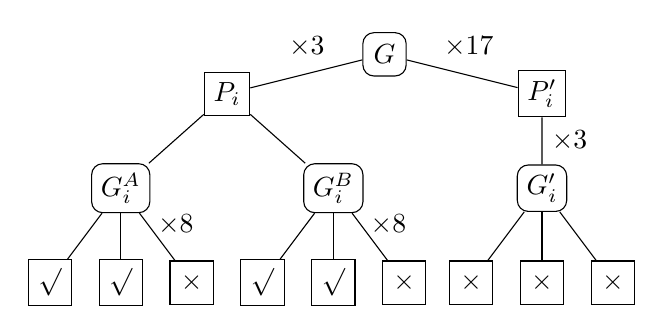
\begin{tikzpicture}[level distance=1.2cm]

\tikzstyle{planbox}=[draw,minimum height=0.55cm,minimum width=0.55cm]
\tikzstyle{goalbox}=[draw,rounded corners,minimum height=0.55cm,minimum width=0.55cm]

\tikzstyle{level 1}=[sibling distance=4cm,level distance=0.5cm] 
\tikzstyle{level 2}=[sibling distance=2.7cm,level distance=1.2cm]
\tikzstyle{level 3}=[sibling distance=.9cm]
\tikzstyle{level 4}=[sibling distance=1cm]

\node[goalbox] (T) {$G$}
   child[solid] {node[planbox] (1) {$P_i$}
      	child {node[goalbox] (11) {$G_i^A$}
			child {node[planbox] {$\surd$}
			}
			child {node[planbox] {$\surd$}
			}
			child {node[planbox] {$\times$}
				edge from parent node[right,near start] {$\times 8$}
			}
	  	}
      	child {node[goalbox] (11) {$G_i^B$}
			child {node[planbox] {$\surd$}
			}
			child {node[planbox] {$\surd$}
			}
			child {node[planbox] {$\times$}
				edge from parent node[right,near start] {$\times 8$}
			}
	  	}
	edge from parent node[above left, near start] {$\times 3$}
   }
   child[solid] {node[planbox] (2) {$P_i'$}
      child {node[goalbox] (22) {$G_i'$} 
	child {node[planbox] {$\times$}}
	child {node[planbox] {$\times$}}
	child {node[planbox] {$\times$}}
	edge from parent node[right] {$\times 3$}
	}
   edge from parent node[above right,near start] {$\times 17$}};

% \draw (T) -- (1) node (aux1) [coordinate,midway]{};
% \draw (T) -- (2) node (aux2) [coordinate,midway]{};
% \draw (aux1) .. controls +(0.3,-0.3) and +(-0.3,-0.3).. (aux2)
% 			node[midway,above] {OR};

% \draw (1) -- (11) node (aux21) [coordinate,midway]{};
% \draw (1) -- (12) node (aux23) [coordinate,midway]{};
% \draw (aux21) .. controls +(0.25,-0.25) and +(-0.25,-0.25).. (aux23)
% 			node[midway,above] {AND};

% \node[below left of=T,text width=2cm,xshift=-3cm] (label)
% 		{$P_i$: plan \\ $G_i$: goals \\ $SG_i$: sub-goals};
\end{tikzpicture}

\end{center}
\caption{Goal-plan tree structure $\T_1$. To succeed, an agent needs 
to make three correct choices, including selecting  $P_i$ at the
top-level. The solutions to $2^3$ worlds are distributed evenly in the $3$ plans 
$P_i$. \CL\ outperforms \BUL\ in this structure.}
\label{fig:T1}
\end{figure}


From our set of experiments, we have selected three hierarchical structures that
best illustrate the results that we have obtained, namely:
% %
\begin{description}
\item[(Tree $\T_1$; Figure~\ref{fig:T1})] For each world state, the
goal has a few plans that can succeed (plans $P_i$), but many other options of comparable
complexity that are bound to fail (plans $P_i'$).\footnote{Here, plan
complexity refers to the size of the fully expanded plan, as represented
by the number of levels of abstraction and the numbers of goals at each level.
The key factor is the number of abstraction levels---abstract plans are not in
themselves complex.}
%%
Under this type of structure, an \CL-based agent will generally perform better 
than an agent using the learning \BUL\ approach.

\item[(Tree $\T_2$; Figure~\ref{fig:T2})] For each world state, the goal has
one plan that can succeed (plan $P$), and a few others that would fail.
However, the plan containing the solution is of substantially
higher-complexity.
%%
In this structure, a \BUL-based agent will outperform an \CL-based one.
% A structure in which \BUL\ is
% expected to have important advantages over \CL, since the latter may wrongly consider a
% top-level plan as a failing plan whereas there is a solution encoded
% under it. 

\item[(Tree $\T_3$; Figure~\ref{fig:T3})] This tree represents a ``balanced''
structure that ends up providing different advantages for both \BUL\ and \CL\ in
different parts of the tree.
\end{description}


% In summary, we found that whereas the agent performance under the \BUL\ and \CL\
% approaches is comparable on the first and third cases, the \BUL\ scheme provides
% substantial benefits in the second case. What is more important, if we consider
% agents that may choose not to consider a plan at all when its chances of success
% are believed very low, then the \CL\ approach collapses completely whereas the
% \BUL\ is robust enough to maintain performance.

% For lack of space, we shall only give the form of tree $\T_1$ and informally
% explain the characteristics of the other two.

Let us next discuss each of the plan-goal structures and how the performance of
\BUL-based and \CL-based agents compare.


Under a structure like $\T_1$, the agent basically has several options of
comparable complexity to resolve the top-level goal $G$ in a certain
world state. In $\T_1$ there are $20$ options.
However, most such options ($17$ in our example, plans $P_i'$)
inevitably lead to failure.  
% %
The benefit of using the \CL\ approach comes from the fact that the agent will
decrease the probability of selecting each of those $17$ failing plans as soon as
they fail for the first time. In contrast, \BUL\ requires multiple failed
experiences of each of those ``bad'' top-level options before decreasing their
probability of selection because each subgoal of each plan $P_i'$ must
be stable before that $P_i'$ is updated. 
%---to update the decision tree of each plan $P_i'$, \BUL\
%requires each of the three subgoals of that plan to be ``stable.''
% %%
The \CL\ agent did indeed perform better in our experiments, in that it
achieved better success rate earlier as shown in Figure~\ref{fig:T1_result}.
% %
% The \CL\ approach reaches $50\%$ success after $600$ iterations,
% whereas it takes more than double that for \BUL.
%%
Observe that, eventually, both approaches will yield optimal
performance.\footnote{Optimal performance in this case amounts to a success rate
of $81\%$, as the environment fails with probability $.1$ for every (working) action and each
successful execution involves the performance of two actions (leaf plans consist
of single actions).}


\begin{figure}[t]
\begin{center}
%!TEX root = ../dsingh-aamas10.tex
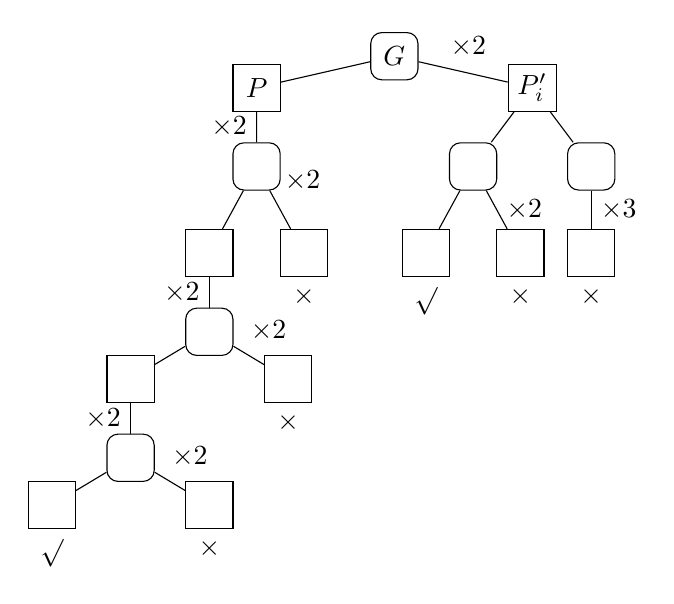
\begin{tikzpicture}[level distance=1.2cm]
\tikzstyle{txt}=[scale=.9]

\tikzstyle{succ}=[label=below:$\surd$]
\tikzstyle{fail}=[label=below:$\times$]


\tikzstyle{planbox}=[draw,minimum height=0.6cm,minimum width=0.6cm]
\tikzstyle{goalbox}=[draw,rounded corners,minimum height=0.6cm,minimum width=0.6cm]

\tikzstyle{level 1}=[sibling distance=3.5cm,level distance=0.4cm] 
\tikzstyle{level 2}=[sibling distance=1.5cm,level distance=1.0cm]
\tikzstyle{level 3}=[sibling distance=1.2cm,level distance=1.1cm]
\tikzstyle{level 4}=[sibling distance=1.2cm,level distance=1.0cm]
\tikzstyle{level 5}=[sibling distance=2.0cm,level distance=0.6cm]
\tikzstyle{level 6}=[sibling distance=1.2cm,level distance=1.0cm]
\tikzstyle{level 7}=[sibling distance=2.0cm,level distance=0.6cm]
\tikzstyle{level 8}=[sibling distance=1.2cm,level distance=1.0cm]

\node[goalbox] (T) {$G$}
   child[solid] {node[planbox] (1) {$P$}
      child {node[goalbox] (11) {\phantom{$G$}}
		child {node[planbox] {\phantom{$P$}}
			child {node[goalbox] {\phantom{$G$}}
				child {node[planbox] {\phantom{$P$}}
					child {node[goalbox] {\phantom{$G$}}
						child {node[planbox,succ] {\phantom{$P$}}}
						child {node[planbox,fail] {\phantom{$P$}}
							edge from parent node[above right,near start] {$\times 2$}
						}
						edge from parent node[left] {$\times 2$}
					}
				}
				child {node[planbox,fail] {$\phantom{P}$}
					edge from parent node[above right,near start] {$\times 2$}
				}
		               edge from parent node[left] {$\times 2$}
			}
		}
		child {node[planbox,fail] {\phantom{$P$}}
			edge from parent node[above right,near start] {$\times 2$}
		}
               edge from parent node[left] {$\times 2$}
	}
   }
   child[solid] {node[planbox] (2) {$P_i'$}
      	child {node[goalbox] (11) {\phantom{$G$}}
			child {node[planbox,succ] {$\phantom{P}$}}
			child {node[planbox,fail] {$\phantom{P}$} 
		               edge from parent node[right] {$\times 2$}
			}
	}
      	child {node[goalbox] {\phantom{$G$}}
			child {node[planbox,fail] {$\phantom{P}$} 
		               edge from parent node[right] {$\times 3$}
			}
	}
	edge from parent node[above right, near start] {$\times 2$}
};
\end{tikzpicture}



\end{center}
\caption{Goal-plan tree hierarchical structure $\T_2$. Successful execution requires numerous correct choices including $8$ correct action nodes. The solutions to $2^3$ worlds are in the plan labelled $P$. \BUL\ outperforms \CL\ in this structure.}
\label{fig:T2}
\end{figure}


\begin{figure*}[t]
\begin{center}
\subfigure[Structure $\T_1$]{\label{fig:T1_result}
%!TEX root = ../dsingh-aamas10-poster.tex
\begin{tikzpicture}[x= 0.008cm,y=9cm]
	\definecolor{darkblue}{rgb}{0.1,0.1,0.5}
	\definecolor{darkred}{rgb}{0.8,0.0,0.1}
    % Draw the axes and grid lines
    \draw[-] (0,0) -- (0,1) -- (2000,1) -- (2000,0) -- cycle; 
    \draw[-,thin, dotted, ystep=0.2, xstep=2000] (0,0) grid (2000,1);
    \foreach \x in {500, 1000, 1500}  \draw [-,xshift=0](\x,4pt) -- (\x,-1pt);
    \foreach \y in {0.0,0.2,0.4,0.6,0.8,1.0}  \draw [-,yshift=0](4pt,\y) -- (-1pt,\y);
    \foreach \x/\xtext in {500/500, 1000/1000, 1500/1500} \node at (\x,0) [below] {\xtext};
    \foreach \y/\ytext in {0.0,0.2,0.4,0.6,0.8,1.0}  \node at (0,\y) [left] {\ytext};
    \node at (0,1.15) {Success};
    \node at (1650,0.1) {Iterations};
    \draw[-,darkred] plot[mark=x,mark size=10,mark options={color=darkred}] 
			file {figs/data/test01v3gm.CP.tikzdata};
    \draw[-,darkblue] plot[mark=o,mark size=6,mark options={color=darkblue}] 
			file {figs/data/test01v3gm.SP.tikzdata};
    % Also draw the expected convergence: 0.9^4 actions=0.6561
    \draw[dashed,-,yshift=0](0,0.81) -- (2000,0.81);
	\node at (2300,0.5) {$\mathcal{T}1$};
\end{tikzpicture}

}
\qquad
\subfigure[Structure $\T_2$]{\label{fig:T2_result}
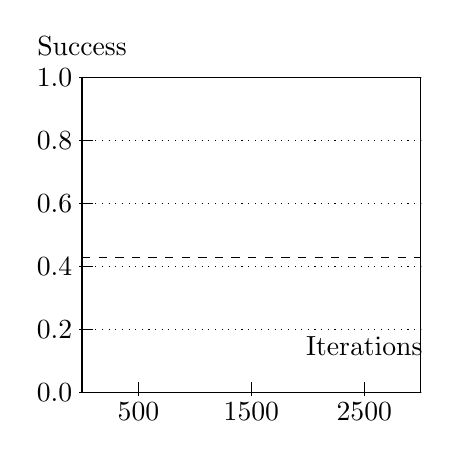
\begin{tikzpicture}[x=0.00143cm,y=4cm]
    % Draw the axes and grid lines
    \draw[-] (0,0) -- (0,1) -- (3000,1) -- (3000,0) -- cycle; 
    \draw[-,thin, dotted, ystep=0.2, xstep=3000] (0,0) grid (3000,1);
    \foreach \x in {500, 1500, 2500}  \draw [-,xshift=0](\x,4pt) -- (\x,-1pt);
    \foreach \y in {0.0,0.2,0.4,0.6,0.8,1.0}  \draw [-,yshift=0](4pt,\y) -- (-1pt,\y);
    \foreach \x/\xtext in {500/500, 1500/1500, 2500/2500} \node at (\x,0) [below] {$\xtext$};
    \foreach \y/\ytext in {0.0,0.2,0.4,0.6,0.8,1.0}  \node at (0,\y) [left] {$\ytext$};
    \node at (0,1.1) {Success};
    \node at (2500,0.15) {Iterations};
    \draw[-] plot[mark=triangle,gray,mark size=3,mark options={color=gray}] 
			file {data/test05v3gm.CP.tikzdata};
    \draw[-] plot[mark=o,gray,mark size=2,mark options={color=gray}] 
			file {data/test05v3gm.SP.tikzdata};
    % Also draw the expected convergence: 0.9^8 actions=0.43046
    \draw[dashed,-,yshift=0](0,0.43046) -- (3000,0.43046);

\end{tikzpicture}

}
\qquad
\subfigure[Structure $\T_3$]{\label{fig:T3_result}
%!TEX root = ../dsingh-aamas10-poster.tex
\begin{tikzpicture}[x=0.0032cm,y=9cm]
    % Draw the axes and grid lines
    \draw[-] (0,0) -- (0,1) -- (5000,1) -- (5000,0) -- cycle; 
    \draw[-,thin, dotted, ystep=0.2, xstep=5000] (0,0) grid (5000,1);
    \foreach \x in {1000, 2500, 4000}  \draw [-,xshift=0](\x,4pt) -- (\x,-1pt);
    \foreach \y in {0.0,0.2,0.4,0.6,0.8,1.0}  \draw [-,yshift=0](4pt,\y) -- (-1pt,\y);
    \foreach \x/\xtext in {1000/1000, 2500/2500, 4000/4000} \node at (\x,0) [below] {\xtext};
    \foreach \y/\ytext in {0.0,0.2,0.4,0.6,0.8,1.0}  \node at (0,\y) [left] {\ytext};
    \node at (0,1.15) {Success};
    \node at (4150,0.1) {Iterations};
    \draw[-,red] plot[mark=x,mark size=10,mark options={color=red}] 
			file {figs/data/testImpactvars2.CP.tikzdata};
    \draw[-,blue] plot[mark=o,mark size=6,mark options={color=blue}] 
			file {figs/data/testImpactvars2.SP.tikzdata};
    % Also draw the expected convergence: 0.9^4 actions=0.6561
    \draw[dashed,-,yshift=0](0,0.6561) -- (5000,0.6561);
	\node at (5700,0.5) {$\mathcal{T}3$};

\end{tikzpicture}

}
\caption{Agent performance under \BUL\ (circles) and \CL\ (crosses) schemes.
Each point represents results from $5$ experiment runs using an averaging window
of $100$ samples. The dashed line represents optimal performance (Note that
outcomes are always $0$ or $1$ so more than expected consecutive successes may
seems like ``above'' optimal performance when averaged).}
\end{center}
\end{figure*}


Let us now analyse the goal-plan tree $\T_2$ shown in Figure~\ref{fig:T2}.
% %
Under such a structure, all successful executions are encoded in a complex plan,
in our case plan $P$. Other options that the agent may have (e.g., plans $P_i'$)
are of less complexity, but do not lead to solutions for resolving the
goal.\footnote{This is an extreme case for illustrative purposes. Of course the
simpler plans $P_i'$ would, in a real program, lead to a solution in some world
states or it would not make sense to include them. The same effect would however
arise if most world states had solutions only in a complex plan branch.}
% %
Because the plan containing the solution, namely $P$, is fairly complex, there
are many ways the agent may fail when exploring the decomposition of $P$. The
agent needs to make several correct choices to obtain a successful execution.
% %
Although we expected \BUL\ to yield better agent performance than \CL, the
difference was enormous in our experiments. Figure~\ref{fig:T2_result} shows that
while the \BUL\ approach achieves optimal performance, which amounts to slightly
over $40\%$ rate of success, in slightly more than $500$ iterations, the \CL\
scheme, requires more than $3000$ execution experiences. The reason is clear:
since there are more chances to fail plan $P$ initially, \CL\ marks this plan as
``bad,'' compared with the non-working plans $P_i'$. On the other hand, \BUL\
would not jump to the conclusion that $P$ is a ``bad'' plan even when failing it,
since it is aware that decisions made below $P$ were not sufficiently informed.
Consequently, plan $P$ will continue to be explored with \emph{equal} likelihood
to plans $P_i'$.
% %
This structure shows exactly the problem discussed in the previous section,
namely, the drawbacks of assuming that a plan is a bad option just because it
happened to fail, without consideration of the confidence in the choices made
below it.


Finally, consider the hierarchical structure $\T_3$ depicted in Figure
\ref{fig:T3}.
% %
In this case, the top-level goal $G$ has four relevant plans, which are all
``complex,'' that is, they all have several levels and multiple goals and plans.
However, given a world state, only one particular path in this hierarchy will
lead to a successful execution (of course, for different states, different
top-level plans may apply). Among other things, this means that at the top-level
the agent needs to select the right plan given the current world state. All 
other plans are bound to eventually fail.
% %
We argue that this is a common feature found in many BDI agent applications, in
that even though the agent has been programmed with several strategies for
resolving a goal, each one is crafted to cover uniquely a particular subset of
states. In other words, these are systems with low \emph{know-how} overlap.
% %
With respect to the two learning approaches we are considering, structure $\T_3$
provides advantages for both of them, in different parts of the tree. The \CL\
scheme is expected to learn faster the inadequacy of the non-working top-level
programs, whereas the \BUL\ would better explore, and find a solution, within the
working top-level plan. This balance is evident in Figure~\ref{fig:T3_result} 
where both approaches show comparable performance.




\subsection{Plan Applicability and Optimality}

So far, we have assumed that the agent considers all relevant plans
for a goal as also \emph{applicable}, even though some may have a very
low chance of success.
% %
This implies that, in contrast with standard BDI systems, our extended
learning BDI framework will \emph{always} select a plan among the relevant
options.
% %
Because executing a plan is often not cost-free in real systems, it is likely
that an adequate plan selection mechanism would in fact \emph{not} execute plans
with too low a probability of success. This, in turn, implies that the system
may, at some point, decide to fail a goal without even trying it, if it
considers that the high likelihood of failure does not justify the
cost of attempting any of the relevant plans.
%cost of failing at that point is preferable to expected
%benefits of executing some available plan.
%%
This is exactly what standard BDI systems do. When no applicable plan
is found for a certain event goal, that event goal is failed right away.


To understand the impact of applicability in our BDI learning framework, we
modified the probabilistic plan selection so that the agent does \emph{not} consider
plans whose chances of success are deemed below a threshold; in our case we set
this threshold to $0.2$.
% %
For simplicity, we  removed the non-determinism in the model of the
environment: actions either fail or succeed in each world state.

%The difference between \CL-based and \BUL-based agents performance when run with
%an applicability threshold could be striking
% %
Using the structure $\T_3$ we found that whereas the \BUL\ scheme maintains its
performance (and in fact may slightly improve due to truly failing leaf plans
being ruled out earlier), the \CL\ approach may not able to learn at all and
could end up eventually failing the top-level goal \emph{always}. This is
reported in Figure~\ref{fig:performance-applicability} (dotted lines).

The explanation for this undesirable behavior under \CL\ is as follows.
% %
Initially, the agent tries all top-level plans for the top-level goal, including
the ones containing potential successful executions. Because of their complexity,
the chance of finding a successful execution immediately is very low, and most
executions fail initially. With each failure, \CL\ decreases the feasibility of
all plans tried, including the top-level one.  After several failures, all plans
for the top-level goal eventually go below the applicability threshold of the
system (including the ``good'' plans). When that happens, the system has no more
applicable plans for the goal and will therefore fail it always.
% %
This behavior does not arise in the original system, because even if all plans
perform very poorly, the agent would always pick one anyway, the successful path
would be eventually be found, and the context decision trees of the plans
associated with such a path would then start ``recovering.''


The reason \BUL\ exhibits more robust behaviour here is that false negative
executions (i.e., failing executions of plans that do encode successful
runs) will \emph{not} be recorded.
% %
The \BUL\ approach relies on a \emph{confidence} test---stability---that checks
whether we are sufficiently well informed to trust that the current failure is
indicative of future attempts.
% %
In the next section, we explore an alternative approach to confidence 
that takes account of how sure we are of the decision tree when we use
it, rather than using stability as a confidence measure for deciding when to record.
%that can be combined with \CL\ (or \BUL) and is able to overcome the
%weaknesses shown here.
